\subsection{Convert Indexed to Float}
    \label{sec:primitiveops_conv2float}
    After computing a reproducible indexed sum, we need to reproducibly and
    accurately convert the result to a single floating point number. There
    are two sources of error in the final floating point sum
    produced by ReproBLAS. The first is from the creation of the indexed sum
    (analyzed in \cite{repsum}). The second is from the conversion from indexed
    sum to floating point number (evaluation of  \eqref{eq:indexedvalue}).
    Because \cite{repsum} guarantees that all fields in the indexed type are
    reproducible, as long as the fields are operated on deterministically
    by the final conversion back to original floating-point format,
    any method to evaluate  \eqref{eq:indexedvalue} accurately and without
    unnecessary overflow or underflow is suitable.

    Assume that $Y$ is the indexed sum of some $x_0, ..., x_{n - 1} \in \F$ (for now, assume no exceptional values). If
    we simply evaluate \eqref{eq:indexedvalue} in an arbitrary order and apply
    the standard summation error bound given by \cite{higham}, the error in the
    final answer $\overline{\mathcal{Y}}$ (the computed floating point
    approximation of $\mathcal{Y}$) is only bounded by (using
    \eqref{eq:baderrorapprox})
    \begin{equation}
      |\overline{\mathcal{Y}} - \sum_{j=0}^{n-1}x_j| \leq n \bigl(2^{W  (1 - K)} + (2  K - 1)  \epsilon\bigr)\max|x_j|
      \label{eq:baderrorapproxdup}
    \end{equation}
    However, if we sum the primary and carry fields in order of decreasing ``unnormalized''
    exponent, the error is bounded by (using  \eqref{eq:errorapprox})
    \begin{equation}
      |\overline{\mathcal{Y}} - \sum_{j=0}^{n-1}x_j| \leq n 2^{W  (1 - K)}\max|x_j|  + 7 \epsilon \bigl|\sum\limits_{j = 0}^{n - 1} x_j\bigr|
      \label{eq:errorapproxdup}
    \end{equation}
    which as we will see can be orders of magnitude smaller than the bound in \eqref{eq:baderrorapproxdup}

    When adding the primary and carry fields it is not necessary to examine the values in the
    fields or sort them explicitly. Their ``unnormalized'' exponent does not
    depend on their values, and their ``unnormalized'' exponents have a
    predetermined order. There is therefore little difference in computational cost between the two methods. They require the same number of
    additions (namely $2 K$), but summing in order requires more conditional branches. However, showing that the
    fields have a certain ordering and that the stronger bound \eqref{eq:errorapproxdup} applies requires
    extensive analysis.

    To further motivate the new conversion algorithm, we compare both the above
    error bounds for indexed summation to an approximated standard error bound
    obtained through standard (recursive) summation of $x_0, ..., x_{n - 1}$ in
    some arbitrary order (given by \cite{higham})
    \begin{equation}
      |S_n - \sum_{j=0}^{n-1}x_j| \leq n \epsilon  \sum\limits_{j = 0}^{n - 1}|x_j| \leq n^2  \epsilon  \max|x_j|
      \label{eq:naiveerrorapproxdup}
    \end{equation}

    Figure \ref{fig:conversionmotivation} compares these three approximate error bounds
    for $K=3$, $W=40$ and double precision $p=53$.
    Note that the term $7 \epsilon |\sum\limits_{j = 0}^{n - 1}x_j|$ is only
    $7$ times larger than the smallest possible error from rounding the
    exact sum of the $x_j$ to the nearest floating point value. To compare the other terms, bound \eqref{eq:errorapproxdup} grows like $2^{-80}n\max|x_j|$,
    whereas bound \eqref{eq:baderrorapproxdup} grows like $5\epsilon n \max|x_j| = 5 \cdot 2^{-53}n\max|x_j|$, which is approximately $8$ orders of magnitude larger.
    Note that in this comparison we bound $\sum_{j=0}^{n-1} |x_j|$ by $n \max |x_j|$,
    which is the case where the input data are almost equal in magnitude,
    so the error bound of the standard summation \eqref{eq:naiveerrorapproxdup} can grow like $n^2$ instead of $n$ which is much worse than both bounds
    \eqref{eq:errorapproxdup} and \eqref{eq:baderrorapproxdup}
    when the number of input values $n$ is great.
    In cases where $\sum_{j=0}^{n-1} |x_j| \approx n \max |x_j|$, for example
    when there are just a few large values and the others are small, then bounds
    \eqref{eq:naiveerrorapproxdup} and \eqref{eq:baderrorapproxdup} are almost
    of the same order of magnitude, which is still worse than bound \eqref{eq:errorapproxdup}
    by 8 orders of magnitude when the true sum is tiny.

\begin{figure}[H]
\begin{center}
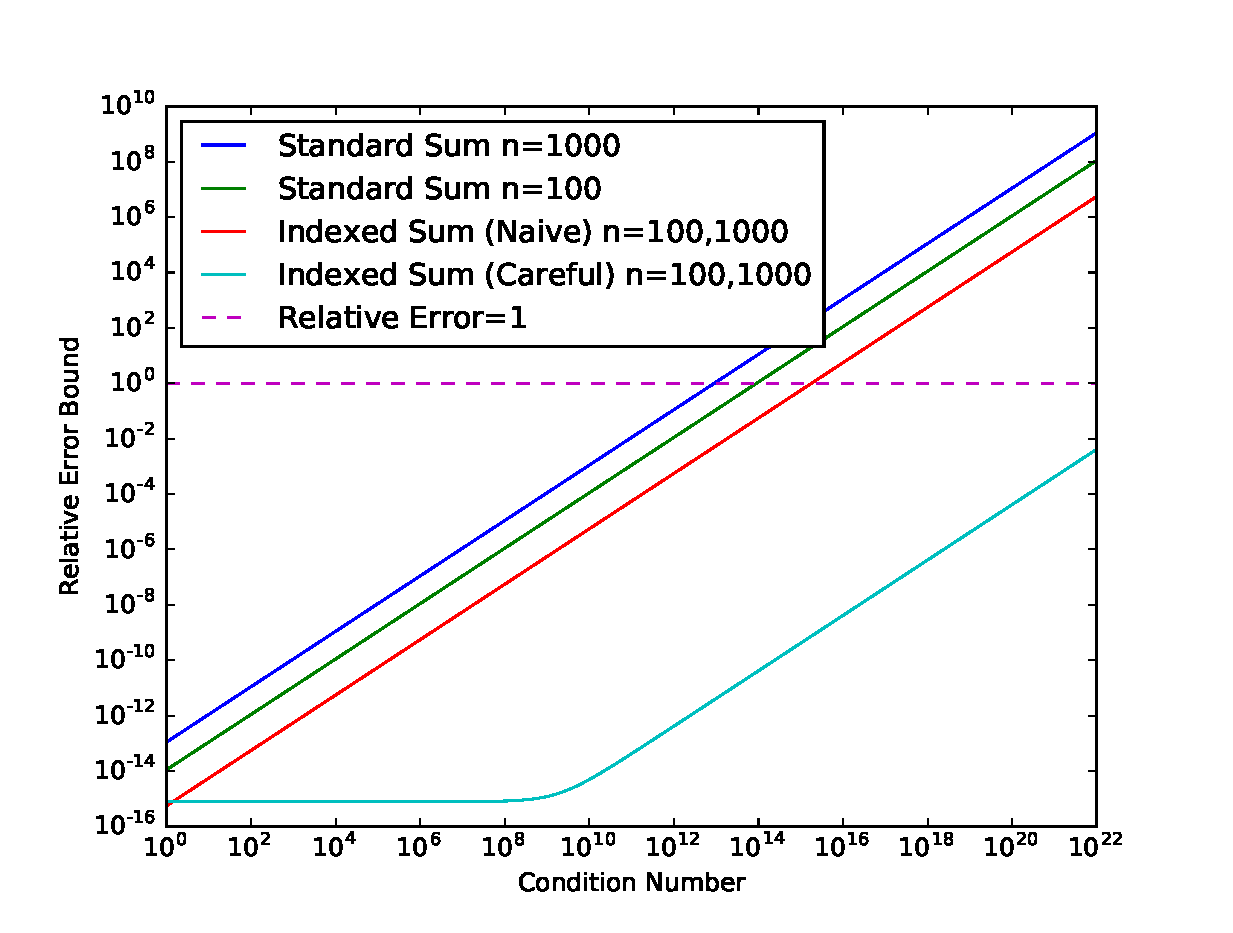
\includegraphics[width=\textwidth]{plots/error_comparison}
\caption{Relative error bounds in calculating $|\sum \limits_{j = 0}^{n - 1}
x_j|$ for different condition numbers (which we define as $\frac{n \cdot \max
|x_j|)}{|\sum \limits_{j = 0}^{n - 1} x_j|}$) of the sum. It is assumed that we
sum using \texttt{double}, $K = 3$, and $W = 40$. ``Indexed Summation
(Careful)'' corresponds to \eqref{eq:errorapproxdup}. ``Indexed Summation
(Naive)'' corresponds to \eqref{eq:baderrorapproxdup}. ``Standard Summation''
corresponds to \eqref{eq:naiveerrorapproxdup} and due to a dependence on $n$
multiple error bounds are shown.}
\label{fig:conversionmotivation}
\end{center}
\end{figure}

    Next we show how to interpret the fields as unnormalized floating point numbers,
    and sort their exponents independently of the actual values of the fields.
    Note that this interpretation is to support reasoning about the conversion algorithm
    presented below, and does not affect the representation format of the data itself
    since IEEE floating-point formats do not permit unnormalized numbers
    beside exceptional values and denormalized numbers.
    Consider a $K$-fold indexed type $Y$ of index $I$.
    Each value ${\mathcal{Y}_k}_P$ in a primary field ${Y_k}_P$ is represented by an offset from $1.5  \epsilon^{-1}  2^{a_{I + k}}$ and ${Y_k}_P \in (\epsilon^{-1}  2^{a_{I + k}}, 2  \epsilon^{-1}  2^{a_{I + k}})$, ${\mathcal{Y}_k}_P$ can be expressed exactly using an unnormalized floating point number ${\mathcal{Y}'_P}_k$ with an exponent of $a_{I + k} + p - 1$.
    As each carry field ${Y_k}_C$ is a count of renormalization adjustments later scaled by $0.25  \epsilon^{-1}  2^{a_{I + k}}$, ${\mathcal{Y}_k}_C$ can be expressed exactly using an unnormalized floating point number ${\mathcal{Y}'_k}_C$ with an exponent of $a_{I + k} + 2  p - 3$.

    First, we have $\exp({\mathcal{Y}'_k}_P) > \exp({\mathcal{Y}'_{k+1}}_P)$ and $\exp({\mathcal{Y}'_{k}}_C) > \exp({\mathcal{Y}'_{k+1}}_C)$ because $a_{I + k} > a_{I + k+1}$.

    Next, note that
    \begin{equation*}
      \exp({\mathcal{Y}'_k}_C) = a_{I + k} + 2  p - 3
    \end{equation*}

    and
    \begin{equation*}
      \exp({\mathcal{Y}'_{k - 1}}_P) = a_{I + k - 1} + p - 1 = a_{I + k} + W + p - 1
    \end{equation*}

    Therefore $\exp({\mathcal{Y}'_k}_C) > \exp({\mathcal{Y}'_{k - 1}}_P)$ because $W < p - 2$.

    Finally, note that
    \begin{equation*}
      \exp({\mathcal{Y}'_{k - 2}}_P) = a_{I + k - 1} + p - 1 = a_{I + k} + 2 W + p - 1
    \end{equation*}

    Therefore $\exp({\mathcal{Y}'_k}_C) < \exp({\mathcal{Y}'_{k - 2}}_P)$ because $2  W > p + 1$.

    Combining the above inequalities, we see that the exponents of all the ${\mathcal{Y}'_k}_P$ and ${\mathcal{Y}'_k}_C$ are distinct and can be sorted as follows:

    \begin{alignat*}{5}
    \exp({\mathcal{Y}'_0}_C) &> \exp({\mathcal{Y}'_1}_C) &&> \exp({\mathcal{Y}'_0}_P) &&> \exp({\mathcal{Y}'_2}_C) &&> \exp({\mathcal{Y}'_1}_P) &&> ... \\
    ... &> \exp({\mathcal{Y}'_k}_C) &&> \exp({\mathcal{Y}'_{k - 1}}_P) &&> \exp({\mathcal{Y}'_{k + 1}}_C) &&> \exp({\mathcal{Y}'_k}_P) &&> ... \\
    ... &> \exp({\mathcal{Y}'_{K - 2}}_C) &&> \exp({\mathcal{Y}'_{K - 3}}_P) &&> \exp({\mathcal{Y}'_{K - 1}}_C) &&> \exp({\mathcal{Y}'_{K - 2}}_P) &&> \exp({\mathcal{Y}'_{K - 1}}_P)
    \end{alignat*}


    These unnormalized floating point numbers may, for convenience of notation,
    be referred to in decreasing order of unnormalized exponent as $\gamma'_0,
    ..., \gamma'_{2  K - 1}$.

    We have just shown that
    \begin{equation}
      \exp(\gamma_0') > ... > \exp(\gamma_{2  K - 1}')
      \label{eq:gammadecreases}
    \end{equation}
    where $\gamma_j$ denotes the normalized representation of the $\gamma'_j$.
    It should be noted that $\gamma_j = \gamma'_j$ as real numbers and that
    $\exp(\gamma_j) \leq \exp(\gamma'_j)$.

    It should be noted that if $\gamma_j$ is a primary field, then either
    $\gamma_{j + 1}$ or $\gamma_{j + 2}$ is a primary field (with the exception of $\gamma_{2K-1}$).
    If $\gamma_j$ is a
    carry field, then either $\gamma_{j + 1}$ or $\gamma_{j + 2}$ is a carry
    field (with the exception of $\gamma_{2  K - 3}$,
    but in this case, suppose that $p \geq 5$ which is true for both IEEE double and single precision,
    we have
    \(
        \exp(\gamma_{2  K - 3}')
        = a_{I + K - 1} + 2  p - 3 \geq a_{I + K - 1} + p + \lceil\frac{p + 1}{2}\rceil - 1
        = \exp(\gamma_{2  K - 1}') + \lceil\frac{p + 1}{2}\rceil
    \)
    ).
    Therefore, as $2  W > p + 1$, for all $j \in \{0, ..., 2K - 3\}$
    \begin{equation}
      \exp(\gamma_j') \geq \exp(\gamma_{j + 2}') + W \geq \exp(\gamma_{j + 2}') + \left\lceil\frac{p + 1}{2}\right\rceil
      \label{eq:gammadecreasesfast}
    \end{equation}

    It should be noted that the ${\mathcal{Y}'_k}_P$ and the
    ${\mathcal{Y}'_k}_C$ can be expressed exactly using floating point types of
    the same precision as ${Y_k}_P$ and ${Y_k}_C$ (except in the case of
    overflow, in which a scaled version may be obtained), and such exact
    floating point representations can be obtained using  \eqref{eq:pri} and
    \eqref{eq:car}.

    Now that we know how to obtain sorted, possibly scaled, fields in order of
    decreasing unnormalized exponent, we explain how to sum them while avoiding
    overflow. We will refer to the floating point type that we use to hold the
    sum during computation as the \textbf{intermediate} floating point type.
    Such a type must have at least as much precision and exponent range as the
    original floating point type.

    Notice that $|\gamma'_0| = |{\mathcal{Y}'_0}_C| < 2 \cdot 2^{\exp({\mathcal{Y}'_0}_C)} = 2 \cdot 2^{e_{\max} + 1 - W + 2  p - 3}$ and $\exp(\gamma'_0) > ... > \exp(\gamma'_{2  K - 1})$.  Therefore $|\gamma'_j| \leq 2^{e_{\max} - W + 2  p - 1 - j}$. The absolute value represented by an indexed type can therefore be bounded by

    \begin{equation}
      \label{eq:maxindexedvalue}
      \sum\limits_{j = 0}^{2  K - 1} |\gamma_j| < \sum\limits_{j = 0}^{2  K - 1} 2^{e_{\max} - W + 2  p - 1 - j} < \sum\limits_{j = 0}^{\infty} 2^{e_{\max} - W + 2  p - 1 - j} = 2^{e_{\max} - W + 2  p}
    \end{equation}

    If the intermediate floating point type has a maximum exponent greater than
    or equal to $e_{\max} - W + 2  p - 1 > e_{\max}$, then no special cases to guard
    against overflow are needed.

    Algorithm \ref{alg:conv2float} represents a conversion routine in such a case.

    \begin{samepage}
    \begin{alg}
      Convert $K$-fold indexed type $Y$ of index $I$ to floating point $x$.
      Here, $z$ is a floating point type with at least the original precision
      and maximum exponent $E_{\max}$ greater than $e_{\max} - W + 2  p$
      \begin{algorithmic}[1]
        \Function{ConvertIndexedToFloat}{K, x, Y}
          \If {${\mathcal{Y}_0}_P$ is 0, \texttt{NaN} or $\pm \texttt{Inf}$}
            \State $x = {\mathcal{Y}_0}_P$
            \State \Return
          \EndIf
          \State $z = {\mathcal{Y}_0}_C$
          \For{$k = 1 \To K - 1$}
            \State $z = z + {\mathcal{Y}_k}_C$
            \State $z = z + {\mathcal{Y}_{k - 1}}_P$
          \EndFor
          \State $z = z + {\mathcal{Y}_{K - 1}}_P$
          \State $x = z$ \label{alg:conv2float:conv}
        \EndFunction
      \end{algorithmic}
      \label{alg:conv2float}
    \end{alg}
    \end{samepage}

    As explained in Section~\ref{sec:indexed}, a value of $0$ in the primary field
    of the first bin means that no numbers have been added to $Y$.
    In addition, as explained in Section~\ref{sec:primitiveops_deposit}, exceptional values
    (\texttt{NaN}, $\pm \texttt{Inf}$) are added directly to the primary field
    of the first bin ${Y_0}_P$. Therefore, exceptional values are reproducibly
    propagated through ${Y_0}_P$, which will be returned as the computed
    result after the final conversion.
    More precisely, a result of \texttt{NaN} means that there is at least
    one \texttt{NaN} in the input or there are both \texttt{Inf} and \texttt{-Inf}
    in the input. A result of $\pm \texttt{Inf}$ means that there is 
    one or more values of $\pm \texttt{Inf}$ of the same sign in the input,
    the rest are of finite value.

    Note that an overflow situation in Algorithm \ref{alg:conv2float} is
    reproducible as the fields in $Y$ are reproducible. $z$ is
    deterministically computed from the fields of $Y$, and the condition that
    $z$ overflows when being converted back to the original floating point type
    in line \ref{alg:conv2float:conv} is reproducible.

    If an intermediate floating point type with exponent greater than or equal
    to $e_{\max} - W + 2  p - 1$ is not available and the lowest bin has index
    0, a rare case, the $\gamma_j$ must be scaled down by some factor during
    addition and the sum scaled back up when subsequent additions can no longer
    effect an overflow situation.

    If the scaled sum is to overflow, then its unscaled value will be greater
    than or equal to $2 \cdot 2^{e_{\max}}$ and it will overflow regardless of
    the values of any ${\mathcal{Y}_k}_P$ or ${\mathcal{Y}_k}_C$ with
    $|{\mathcal{Y}_k}_P| < 0.5 \cdot 2^{-\rho} 2^{e_{\max}}$ or
    $|{\mathcal{Y}_k}_C| < 0.5 \cdot 2^{-\rho}2^{e_{\max}}$ (where $\rho$ is
    the intermediate floating point type's precision). If the floating point
    sum has exponent greater than or equal to $e_{\max}$ these numbers are not
    large enough to have any effect when added to the sum. If the sum has
    exponent less than $e_{\max}$, then additions of these numbers cannot cause
    the exponent of the sum to exceed $e_{\max}$ for similar reasons.

    As the maximum absolute value of the true sum is strictly smaller than
    $2^{e_{\max} - W + 2 p}$, a sufficient scaling factor is $2^{2p-W-2}$,
    meaning that the maximum absolute value of the true scaled sum is
    strictly smaller than $2^{e_{\max}}$ (and since it will be shown
    later that the computed sum is accurate to within a small factor of the
    true sum, the computed sum will stay strictly smaller than $2 \cdot
    2^{e_{\max}}$ and will not overflow.)

    When $\exp(\gamma'_j) < e_{\max} - \rho - 1$, the sum may be scaled back up
    and the remaining numbers added without scaling. Notice that no overflow
    can occur during addition in this algorithm. If an overflow is to occur, it
    will happen only when scaling back up. As the fields in the indexed type
    are reproducible, such an overflow condition is reproducible.

    If the sum is not going to overflow, then the smaller $y'_j$ must be added
    as unscaled numbers to avoid underflow.

    Algorithm \ref{alg:conv2floatoverflow} represents a conversion routine in the case where a floating point type without an expanded exponent is available.

    \begin{samepage}
    \begin{alg}
      Convert a $K$-fold indexed type $Y$ of index $I$ to floating point $x$.
      Here, $z$ is a floating point number with precision $\rho \geq p$
      \begin{algorithmic}[1]
        \Function{ConvertIndexedToFloatNative}{K, x, Y}
          \If {${\mathcal{Y}_0}_C$ is NaN or $\pm$Inf}
            \State $x = {\mathcal{Y}_0}_C$
            \State \Return
          \EndIf
          \State $k = 1$
          \While{$k \leq 2 K$ and $\exp(\gamma_k) \geq e_{\max} - \rho - 1$}
            \State $z = z + (\gamma_k / 2^{2 p - W - 2})$
            \State $k = k + 1$
          \EndWhile
          \State $z = z \cdot 2^{2 p - W - 2}$
          \While{$k \leq 2 K$}
            \State $z = z + \gamma_k$
            \State $k = k + 1$
          \EndWhile
          \State $x = z$
        \EndFunction
      \end{algorithmic}
      \label{alg:conv2floatoverflow}
    \end{alg}
    \end{samepage}

    If an indexed type is composed of \texttt{float}, then \texttt{double}
    provides sufficient precision and exponent to use as an intermediate type
    and Algorithm \ref{alg:conv2float} may be used to convert to a floating
    point number.  However, if an indexed type is composed of \texttt{double},
    many machines may not have any higher precision available. We therefore
    perform the sum using \texttt{double} as an intermediate type. As this does
    not extend the exponent range we must use Algorithm
    \ref{alg:conv2floatoverflow} for the conversion.

    In ReproBLAS, the appropriate conversion for the given data type is available as \texttt{idxd\_xxiconv} in \texttt{idxd.h} (see Section \ref{sec:reproBLAS} for details). This conversion routine sums \texttt{float} with \texttt{double} (using Algorithm \ref{alg:conv2float}) and sums \texttt{double} with \texttt{double} (using Algorithm \ref{alg:conv2floatoverflow}).
